\documentclass[11pt]{article}
\usepackage[utf8]{inputenc} % Para caracteres en espa�ol
\usepackage{amsmath,amsthm,amsfonts,amssymb,amscd}
\usepackage{multirow,booktabs}
\usepackage[table]{xcolor}
\usepackage{fullpage}
\usepackage{lastpage}
\usepackage{enumitem}
\usepackage{multicol}
\usepackage{fancyhdr}
\usepackage{mathrsfs}
\usepackage{wrapfig}
\usepackage{setspace}
\usepackage{esvect}
\usepackage{calc}
\usepackage{multicol}
\usepackage{cancel}
\usepackage{graphicx}
\graphicspath{ {pictures/} }
\usepackage[retainorgcmds]{IEEEtrantools}
\usepackage[margin=3cm]{geometry}
\usepackage{amsmath}
\newlength{\tabcont}
\setlength{\parindent}{0.0in}
\setlength{\parskip}{0.05in}
\usepackage{empheq}
\usepackage{framed}
\usepackage{newtxmath}
\usepackage{euscript}
\DeclareMathAlphabet{\mathpzc}{T1}{pzc}{m}{it}
\usepackage[most]{tcolorbox}
\usepackage{xcolor}
\colorlet{shadecolor}{orange!15}
\parindent 0in
\parskip 12pt
\geometry{margin=1in, headsep=0.25in}
\theoremstyle{definition}
\newtheorem{defn}{Definition}
\newtheorem{reg}{Rule}
\newtheorem{exer}{Exercise}
\newtheorem{note}{Note}
\newcommand{\volume}{{\ooalign{\hfil$V$\hfil\cr\kern0.08em--\hfil\cr}}}
\newcommand{\parr}{\mathbin{\|}} % Parralel Symbol
\begin{document}
\setcounter{section}{0}
\setcounter{page}{2}
\setcounter{equation}{1}
%\definecolor{babyblue}{rgb}{0.54, 0.81, 0.94}
\definecolor{babyblueeyes}{rgb}{0.63, 0.79, 0.95}
\definecolor{babyblue}{rgb}{0.69, 0.88, 0.9}

 \pagestyle{fancy}
\fancyhf{}
\rhead{Section 6:  Ionization}
\rfoot{Page \thepage}
\thispagestyle{empty}

\begin{center}
{\LARGE \bf Section 6:  Ionization}\\
{\large AE435}\\
Spring 2018
\end{center}
\vspace{5mm}
\section{Equilibrium Ionization}
Here we derive the ionization fraction for an equilibrium gas.  This results in what is called the Saha Equation.
\vspace{10mm}
\tableofcontents
\newpage
\subsection{Detailed Balancing}
Assume \textbf{detailed balancing}, where every process is balanced by the reverse process:
 %rate of creating same as rate of destroying that outcome.
   \begin{equation*}
 \begin{aligned}
A + e 	\iff  A^{+} + 2e
 \end{aligned}
 \end{equation*}
 An atom collision with an electron can knock off an electron on the atom creating an ion. 

Examples of the sort of reactions involved in detailed balancing:
\vspace{-5mm} 
  \begin{enumerate}
 \item  Inelastic collision with a 3-body recombination. 
   \begin{equation*}
 \begin{aligned}
\tilde{x} + A \iff x + A^{+} + e
 \end{aligned}
 \end{equation*}
 (A high-energy particle collides with an atom, knocking off an electron turning it into an ion)
 \item Photoionization with radiative recombination
   \begin{equation*}
 \begin{aligned}
hv + A \iff A^{+} + e%photon and particle. photon ionizes particle a, Ionized A and electron
 \end{aligned}
 \end{equation*}
 (A photon-particle collision ionizes the particle by knocking out an electron)
 \end{enumerate}

The overall reaction can be described by an equilibrium constant, a function of pressure and temperature:
   \begin{equation}
 \begin{aligned}
K_{n}(P,T) = \frac{n_{+}n_{e}}{n_{A}}%function or press and temp, numver density of ion and electron over number density of atoms.
 \end{aligned}
 \end{equation}

We can show from statistical mechanics that at equilibrium...
 \begin{shaded}
\textbf{Boltzmann Distribution}
 \begin{equation}
 \begin{aligned}
 \frac{N_{i}}{N} = \frac{n_{i}}{n} = \frac{e^{-\varepsilon_{i}/kT}}{\sum_{i} \, e^{-\varepsilon_{i}/kT}}
 \end{aligned}
 \end{equation}%the macrostate that gives rise to the most possible microstates.
 
Where
 \begin{equation*}
 \begin{aligned}
 N & \text{ is the total population within the control volume} \\ 
 N_{i} & \text{ is the population within the CV at a given state, i} \\ 
 \varepsilon_{i} & \text{ is the energy state ij} \\ 
  k & \text{ is Boltzmann constant.} \\ 
 \end{aligned}
 \end{equation*}
 
 The Boltzmann Distribution is a probability distribution or frequency distribution of particles in a system over various possible states at equilibrium. 
 \end{shaded}

We will use this when moving onto partition functions.


\newpage
\subsection{Partition Functions}
We can define...
 \begin{framed}
 We can define a \textbf{Total Partition Function} for a given species that is the product of a series of individual partial partition functions for all the different energy modes that could exist,
 \begin{equation}
 \begin{aligned}
F = f^t f^e f^r f^v
 \end{aligned}
 \end{equation}
Where for each energy mode of a given species:
 \begin{equation*}
 \begin{aligned}
 f^t & \text{ is the Translational Partial Partition Function} \\ 
f^e & \text{ is the Electronic Partial Partition Function} \\ 
f^r & \text{ is the Rotational Partial Partition Function} \\ 
 f^v & \text{ is the Vibrational Partial Partition Function} \\ 
 \end{aligned}
 \end{equation*}
We have a partial partition function.
 \end{framed}
A \textbf{Partial Partition Function} is given by
 %these tell you how the energy is partisioned or distrbuted across all the available energy states. There are certain translational energy states that an atom can be in and its not continuous. ALl stems from quantum nature of particles. There are discrete bins of energy we can put particles into. 
   \begin{equation}
 \begin{aligned}
f = \sum_i \exp \Bigg(-\frac{ \varepsilon_i}{kT}\Bigg)
 \end{aligned}
 \end{equation}
This tells us how the energy is distributed across any available energy states. There are distributions amongst every form of energy within a system. As an example, the translational energy states of an atom can be different in one area of the system compared to the other. Jahn defines the partial partition function as the sum of accessible energy states, appropriately weighted by degeneracies and by the Boltzmann factors in the relative energies of those states. The Boltzmann factor is that exponential term we see in the Equation 5
 
Other ways of writing the partial partition function include:
   \begin{equation}
 \begin{aligned}
f = \sum_i \exp \Bigg(-\frac{ \varepsilon_i - \varepsilon_o}{kT}\Bigg)
 \end{aligned}
 \end{equation}

where   $\varepsilon_{o}$    	is the ground-state energy. (Note: this is a more general form as it indicates that energy is relative $\varepsilon_{o} = 0$ for atoms and $\varepsilon_{o}=\varepsilon_{i}$ for the ionization energy.                                           
   \begin{equation}
 \begin{aligned}
f = \sum_i g_i \exp \Bigg(-\frac{ \varepsilon_i - \varepsilon_o}{kT}\Bigg)
 \end{aligned}
 \end{equation}
 
includes the degeneracy     $g_{i}$ 	, making it useful for electronic states.%where multiple energy states can have the same energy level.
 \newpage
The partition function is a link between classical thermo and the microscopic behavior of gases (statistical kinetic theory).  It is fairly easy to show that the total energy for N particles is:%
 
   \begin{equation}
 \begin{aligned}
E = NkT^2 \, \frac{\partial}{\partial T} \ln f
 \end{aligned}
 \end{equation}
 
For instance...
\begin{framed}
The \textbf{Translational Partial Partition Function} is given on quantum mechanics basis, as Equation 9 for atoms of mass $M_A$:
   \begin{equation}
 \begin{aligned}
f_A^t = \frac{(2 \pi M_A k T)^{\frac{3}{2}}}{h^3} = K T^{\frac{3}{2}}
 \end{aligned}
 \end{equation}
 
Using Equation 9, we can take the logarithmic derivative to find... 
   \begin{equation}
 \begin{aligned}
 \frac{\partial}{\partial T} \ln f_A^t = \frac{1}{f_A^t}  \, \frac{\partial}{\partial T} f_A^t
 \end{aligned}
 \end{equation}
Such that
   \begin{equation}
 \begin{aligned}
 \frac{\partial}{\partial T} \ln f_A^t = \frac{1}{K T^{\frac{3}{2}}} \, \frac{3}{2} \, K T^{\frac{1}{2}} = \frac{3}{2} \frac{1}{T}
 \end{aligned}
 \end{equation}
 
The total translational energy is then: (substituting equation 11 into equation 8)%substituting 6.11 into 6.8

  \begin{equation}
 \begin{aligned}
E_{tr} = NkT^2 \, \frac{\partial}{\partial T} \ln f_A^t = NkT^2 \, \frac{3}{2} \frac{1}{T} = \frac{3}{2} N k T
 \end{aligned}
 \end{equation} 
 
which is the result we had before in Chapter 4.1.2. when we discussed Kinetic Theory and Internal Translational Energy.
 \end{framed}
We can also find that...
 \begin{framed}
\textbf{electronic partial partition function}
 \begin{equation}
 \begin{aligned}
 f^e = \sum_{j=0}^{n} g_j \exp \Bigg(-\frac{ \varepsilon_j}{kT}\Bigg)
 \end{aligned}
 \end{equation}
Where
 \begin{equation*}
 \begin{aligned}
 g_{i} & \text{ degeneracy for state j} \\ 
 j=0 & \text{ represents the ground state} \\ 
 j=n & \text{ is the highest bound state} \\ 
 \end{aligned}
 \end{equation*}
 \end{framed}
Note that this series converges rapidly, so we only to take the first few terms at low to moderate temperatures.  In hot plasmas, may need to take many terms for an accurate solution. The reason why at low moderate temperatures we can simply take the first two terms is because the energy of each atomic state increases significantly with every orbital. 

Now lets consider a species with negligible rotational and vibrational modes meaning we are only considering atoms or a monatomic species. We can define:
 \begin{shaded}
\textbf{Total Atomic Partition Function}
 %only considering atoms. The model we are developing for is for a monotomic species. 
   \begin{equation}
 \begin{aligned}
F_A = f_A^t f_A^e
 \end{aligned}
 \end{equation}
 
Substituting in the partial partition functions,
   \begin{equation}
 \begin{aligned}
F_A =   \frac{(2 \pi M_A k T)^{\frac{3}{2}}}{h^3} \, \sum_{j=0}^{n} g_j \exp \Bigg(-\frac{ \varepsilon_j}{kT}\Bigg)  %h is plank constant
 \end{aligned}
 \end{equation}
 \end{shaded}
 \vspace{-5mm}
 Likewise,
 \begin{shaded}
 \textbf{Total Ionic Partition Function}
    \begin{equation}
 \begin{aligned}
F_+ = f_+^t f_+^e
 \end{aligned}
 \end{equation}
Substituting in the partial partition functions,
   \begin{equation}
 \begin{aligned}
F_+ =   \frac{(2 \pi M_+ k T)^{\frac{3}{2}}}{h^3} \, \sum_{j=0}^{n} g_j \exp \Bigg(-\frac{ \bar{\varepsilon}_j^+}{kT}\Bigg)  %h is plank constant
 \end{aligned}
 \end{equation}
 \end{shaded}
 \vspace{-5mm}
We need to make sure that we have consistent assumptions about the energy reference state.  Doesn't matter what it is, but it has to be the same for all.
\vspace{-5mm}
\begin{itemize}
\item For atoms, we use the ground state, $\varepsilon_j = 0$
\item For ions, we need to add the ionization energy to reference back to atomic ground, thus...
\end{itemize}

 \begin{shaded}
 \textbf{Ionic Ground State}
     \begin{equation}
 \begin{aligned}
\varepsilon_j^+ = \bar{\varepsilon}_j^+ - \varepsilon_i
 \end{aligned}
 \end{equation}
 
Where the following terms express an electronic energy level in the ion:
     \begin{equation*}
 \begin{aligned}
     \varepsilon_j^+ &= \text{is referenced to the ionic ground state} \\
     \bar{\varepsilon}_j^+ &= \text{is referenced to the atomic ground state} \\
    \varepsilon_i           	&= \text{is the ionization energy (referenced to the atomic ground state)} \\
	 \end{aligned}
 \end{equation*}
 \end{shaded}
\newpage
Finally, we can define at a partition function for free electrons:
 \begin{shaded}
\textbf{Total Electron Partition Function}%electrons cant have electronic energt if they are free. Electronic energy comes from electric potential. No rot energy, no vib. Only translational energy.
     \begin{equation}
 \begin{aligned}
F_e = f_e^+ g_e
 \end{aligned}
 \end{equation}
where        $g_{e }=2$      	is the spin degeneracy (the only internal degree of freedom).

Substituting in the partial partition functions,
    \begin{equation}
 \begin{aligned}
F_e =   \frac{2 \, (2 \pi M_e k T)^{\frac{3}{2}}}{h^3}
 \end{aligned}
 \end{equation}
\end{shaded}
Electrons can't have electronic energy if they are free since electronic energy comes from an electric potential. There is also no rotational or vibrational energy. Free electrons only have translational energy.

So far, we have only looked at monatomic species. Now we are going to combine all of these together using Equation 2 in order to derive the SAHA equation.
\newpage
\subsection{Saha Equation}
The equilibrium constant for ionization as seen from Equation 2 is
\begin{equation}
 \begin{aligned}
K_{n} = \frac{n_{+}n_{e}}{n_{A}}
 \end{aligned}
 \end{equation}
 
which can be expressed as the ratio of total partition functions,

    \begin{equation}
 \begin{aligned}
K_{n} = \frac{F_{+}F_{e}}{F_{A}}
 \end{aligned}
 \end{equation}
 
Substituting in these partial partition functions, we get
     \begin{equation}
 \begin{aligned}
K_n = \frac{2 \, (2 \pi M_e k T)^{\frac{3}{2}}}{h^3} \, \Bigg(\frac{f_+^e}{f_A^e}\Bigg) \, \exp \Bigg(-\frac{ \varepsilon_i}{kT}\Bigg) 
 \end{aligned}
 \end{equation}
\textbf{Question: }Why don't we have translational partition functions for atoms or ions?

\textbf{Answer: } The terms canceled because their masses are about the same. The only difference between the two is in the mass. Understanding that the masses are very similar, the equations are identical and cancel out.

In this equation
     \begin{equation}
 \begin{aligned}
f_+^e = \sum_{j}^{n} g_j^+ \exp \Bigg(-\frac{ \varepsilon_j^+}{kT}
 \end{aligned}
 \end{equation}
 is the electronic partial partition function for ions, and
     \begin{equation}
 \begin{aligned}
f_A^e = \sum_{j}^{n} g_j \exp \Bigg(-\frac{ \varepsilon_j}{kT}
 \end{aligned}
 \end{equation}
 
is  the electronic partial partition function for atoms.  

This is the classic form of the Saha Equation from astrophysics (6.23).
 
An alternative form used often in gas dynamics is started by defining the ionization fraction
 \begin{shaded}
\textbf{Ionization Fraction}
 \begin{equation}
 \begin{aligned}
 \alpha = \frac{n_{+}}{n_{A}^+ n_+} = \frac{n_+}{n_o}%what percent of the gas is ionized when in equillibirum. 
 \end{aligned}
 \end{equation}
Where
 \begin{equation*}
 \begin{aligned}
 n_{+} & \text{ is the ion density} \\ 
 n_{A} & \text{ is the neutral density} \\ 
 n_{o} & \text{ is the total density of heavy particles} \\ 
 \end{aligned}
 \end{equation*}
 \end{shaded}

If we assume quasi-neutrality meaning we have an equal number of positive and negative particles.
    \begin{equation}
 \begin{aligned}
n_+ = n_e
 \end{aligned}
 \end{equation}
Then we can write 

     \begin{equation}
 \begin{aligned}
1 + \alpha = \frac{n_a + n_+ + n_+}{n_o} = \frac{n_a + n_+ + n_e}{n_o}
 \end{aligned}
 \end{equation}
 
Such that the pressure from all 3 species (ions, atoms, electrons) is:

     \begin{equation}
 \begin{aligned}
P = (n_a + n_+ + n_e)\,kT = (1 + \alpha)\,n_okT
 \end{aligned}
 \end{equation}
 
Substituting this into the equilibrium constant from Equation 21  we get:
 \begin{shaded}
\textbf{SAHA Equation}
     \begin{equation}
 \begin{aligned}
\frac{\alpha^2}{1-\alpha^2} = \beta (P,T)%the amount of ionization is dependtent on tepreature and pressure. Higher temp = more ionization, everything has more energy meaning the have more translational energy. Higher pressure = lower ionization becasue we get more 3-body recombinations.
 \end{aligned}
 \end{equation}
where

 \begin{equation}
 \begin{aligned}
\beta (P,T) = \frac{2 \, (2 \pi M_e)^{\frac{3}{2}} \, (kT)^{\frac{5}{2}}}{P\,h^3} \, \Bigg(\frac{f_+^e}{f_A^e}\Bigg) \, \exp \Bigg(-\frac{ \varepsilon_i}{kT}\Bigg) 
 \end{aligned}
 \end{equation}
 
 The amount of ionization is dependent on temperature and pressure. A higher temperature means more ionization, everything has more energy meaning that there will be higher translational energy resulting in more collisions resulting in more electrons being knocked off atoms. Higher pressure equates to lower ionization because we get more three-body recombinations.
 \end{shaded}
 
 \newpage
We can show a plot for argon:

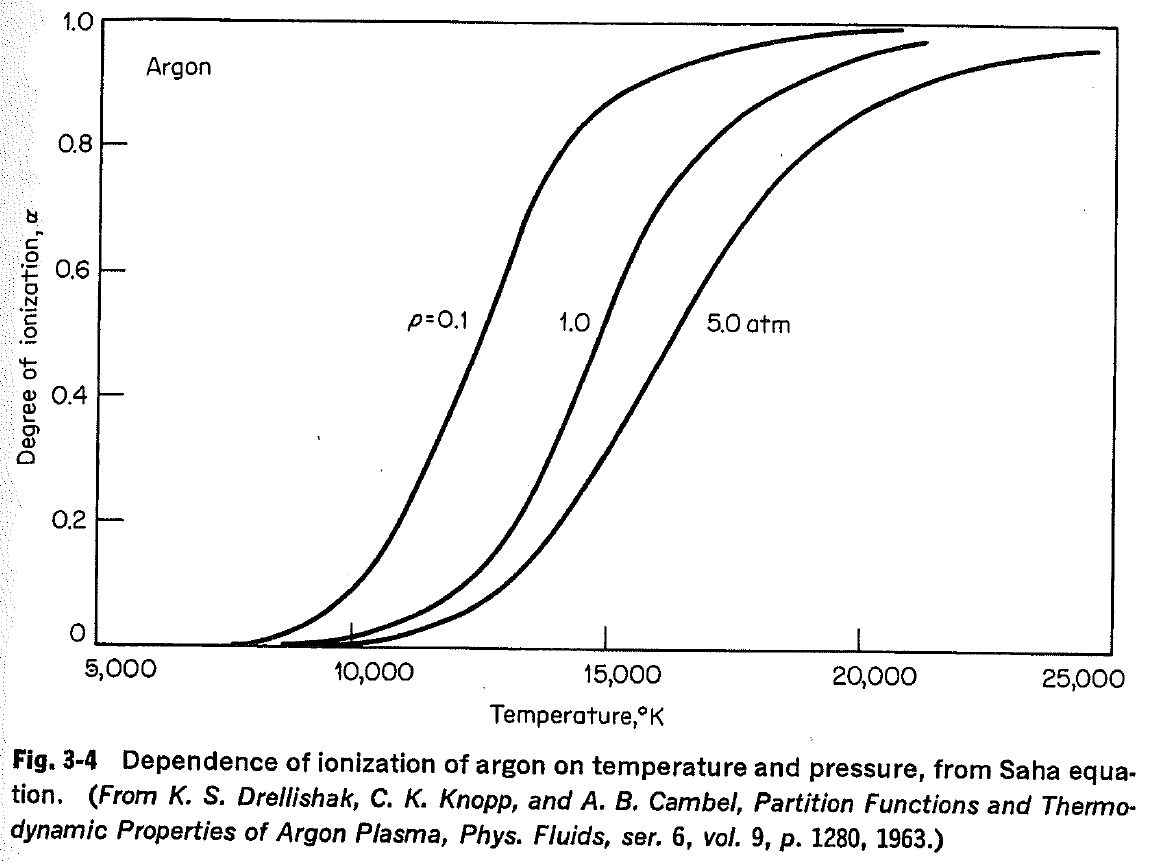
\includegraphics[scale=0.5]{1.png}

%See hw 4 problem 4 for xenon example.
%We see at a fixed temperature, as pressure
 
Note that collisional recombination drives the ionization fraction down at higher pressures.%3-body recombination - argon ion +argon atom+electron goes into 2 argon atoms as the recombinatino. 
 
Jahn gives a more complex analysis, required for multiple species and internal degrees of freedom.  Main points:
\begin{itemize}
\item Vibration and rotation require their associated partition functions
\item Additional reactions (dissociation, etc) can be handled the same way
\item Multiple ionization (high temp, low density) adds partition function and number of reactions
\end{itemize}
\newpage
\subsection{Conditions for Equilibrium}
%this saha equation is on a model based on thermal equillibirum. Lets talk about other models without equillibrium levels of ionization. 
The above analysis assumes \textbf{Complete Thermodynamic Equilibrium (CTE)} meaning we assume:
\begin{enumerate}
\item Single temperature $T_e = T_+ = T_A$
\begin{itemize}
\item All of the species we discussed had the same. The temperature of ions, atoms and electrons was the same as the temperature of the entire gas. In a lot of electric propulsion systems this is rarely the case. Maybe in the case of a magneto-thruster that operates at a higher density plasma, but it still wont be close.
\end{itemize}
\item Homogeneous plasma % No gradiance in P, T, I_{y} (radition field)
\begin{itemize}
\item No gradience in pressure, temperature or radiation field ($I_v$)
\end{itemize}
\item Radiation field follows blackbody distribution
    \begin{equation}
 \begin{aligned}
I_{v} = B_v(T) = \frac{2h\nu^2}{c_o^2}\,\frac{1}{\exp(hv/kt)-1}%radiation intensity
 \end{aligned}
 \end{equation}
where    $I_{\nu}$ 	is the radiation intensity (energy per unit time per unit area per unit solid angle), $\nu$ is the photon frequency and  $c_0$ 	is the vacuum speed of light.  Note that this requires an optically thick plasma, where all radiation is absorbed and re-radiated multiple times (as in Sun's interior).

\vspace{5mm}
 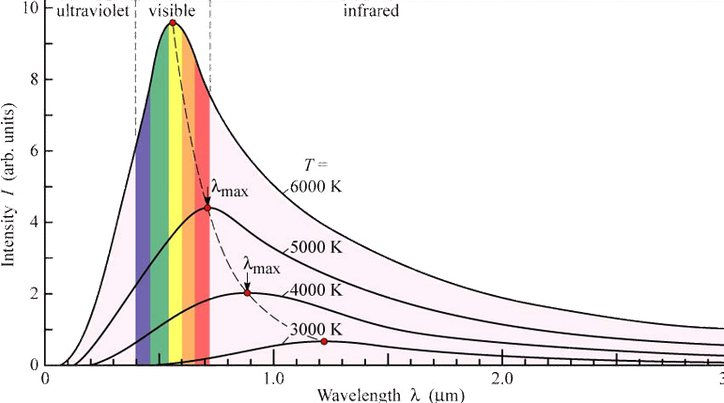
\includegraphics[scale=0.6]{2.png}
 \newpage
\item Maxwellian-Boltzmann Energy Distribution.  
\begin{itemize}
\item Which follows from the Maxwellian velocity (speed) distribution from Chapter 4 Equation 30
\end{itemize}
    \begin{equation}
 \begin{aligned}
\frac{\partial n}{n} = \frac{2 \varepsilon^{\frac{1}{2}}}{\pi^{\frac{1}{2}} \, (kT)^{\frac{3}{2}}} \, \exp \Bigg(-\frac{ \varepsilon_i}{kT}\Bigg) \, \mathrm{d}\varepsilon
 \end{aligned}
 \end{equation}
 \end{enumerate} 
 
For Te = 2eV electrons

  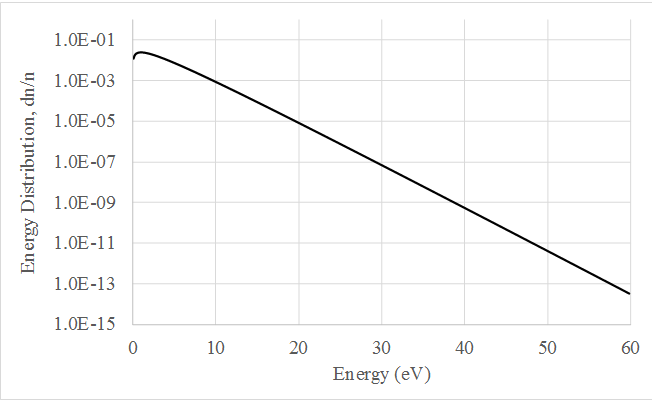
\includegraphics{3.png}
The plot shows the distribution of particles across energy space. 

Note that the slope varies inversely with the temperature, because of $\exp(1/T)$ term in Equation 33.
We use this in several diagnostics (Langmuir probes, atomic Boltzmann method in optical emission spectroscopy) to measure plasma temperature.

Also note the dip in energies less than two times the temperature. This is because the first part of Equation 33 is important whenever the energy is relatively small. It blows up after the exponential term dominates at higher temperatures.
\newpage
In terms of speed,

     \begin{equation}
 \begin{aligned}
\frac{\mathrm{d} n}{n} = \Bigg(\frac{2}{\pi}\Bigg)^{\frac{1}{2}} \, \Bigg(\frac{m}{kT}\Bigg)^{\frac{3}{2}} \, c^2 \, \exp\Bigg(\frac{-mc^2}{2kT}\Bigg) \mathrm{d}c
 \end{aligned}
 \end{equation}
 
And, again, the mean speed for a Maxwellian is:
 
     \begin{equation}
 \begin{aligned}
\bar{c} = \Bigg(\frac{8kT}{\pi m}\Bigg)^{\frac{1}{2}}
 \end{aligned}
 \end{equation}
In CTE,
\begin{itemize}
\item All ionization follows the Saha equation
\item All excitation follows the Boltzmann equation
\end{itemize}
 
 
\subsubsection{Deviations from Equilibrium} %other models for ionization without thermal equillibrium.
\begin{enumerate}
    \item Local thermodynamic equilibrium (LTE), where plasma is
    \begin{itemize}
        \item Sufficiently dense that collisions are dominant populating mechanism %particle will go from ground to ionized, casued by collision.
        \item Optically thin, so radiation field is nonequilibrium, can't use Planck's law %all radiation leaves the plasma, does not get reapbsorbed somewhere else. Does not get absorbed anywhere else. Now the...
        \item Radiative processes do not follow detailed balancing, assume we can ignore radiation processes, plasma is collision determined.%the process that created the photon lacks the balance to take it back. 
    \end{itemize}
    In LTE, radiative emission dominates over absorption and photoionization, depleting the number of free electrons and excited states.  LTE is frequently encountered in lab plasmas.%Pretty common assumption.
    \item Partial local thermodynamic equilibrium (PLTE), where plasma is lower density:
    \begin{itemize}
    	\item Collisions are in detailed balance for upper energy levels %
    	\item Collisions are not in detailed balance for transitions to the ground state%what is goign to happen is the ground state is over populated, density is not high enough to move to a higher lever. We have an excess of particles in ground states.
    	\item Often Ti < Te %As a result we have a temperature difference between ions and electrons. 
    \end{itemize}
    As a result, upper energy levels follow Boltzmann distribution, but the ground state is overpopulated.  Again, depletes the free electron density.
    \item Non-equilibrium Plasma
    \begin{itemize}
    \item Multi-thermal "equilibrium"
    where we have a two-temperature plasma.  Typically:
         \begin{equation*}
 \begin{aligned}
T_{e} > or > > T_{i} \approx T_{A}
 \end{aligned}
 \end{equation*}
    The reason for this difference in temperatures is via electron-impact collisions are an efficient method to transfer energy to gas, but a poor method of transferring momentum.  So atoms get energy from electron to become ionized (takes ionization energy), but they don't get momentum, so their translational energy (temperature) doesn't change. 
     %Good for ionizing the gas or moving electrons to exicted states but not good at transfereing momementum to the atom becasue electrons are much much smaller than atoms/ions.
    Fluorescent lights work by electron-impact excitation of mercury atoms.  (The dominant lines are in the UV, but coatings in the tube walls downconvert to visible light).  Temperatures:
    \begin{itemize}
        \item Gas, 300 K ~ 1/40 eV
        \item Electrons, 3.5 eV ~ 35,000 K
    \end{itemize}
    Collisional processes are often dominated by electrons, so we can get LTE or PLTE where the relevant temperature is Te.
    \item Corona "equilibrium"
    Not really a true equilibrium, as there is no detailed balancing.  Characteristics:
    \begin{itemize}
        \item Very low density plasmas
        \item Radiative decay rates >> collisional decay rates %meaning if there is a collision that happens that exictes an electron. Another collision could get knocked off. But here a collision is so infrewuency that when a collisiton happens and exites an electron, the times between the next collisiosn will be so long that the electron radiates aways.
        \item Optically thin
        \item Radiative excitation and ionization << collisional excitation and ionization%particles are becoming excited via collisions, not vecasue of radiation.
    \end{itemize}
    In this case we can balance
    
    Energy in by collisions = energy out by radiation
    
    For charge states Z and Z+1, the ionization balance is then:
         \begin{equation*}
 \begin{aligned}
n_e n_{z+1} k_r = n_e n_z k_c
 \end{aligned}
 \end{equation*}
    where
            \begin{equation*}
 \begin{aligned} 
             k_r &=\text{is the radiative recombination rate [$s^{-1}$]}\\
             k_c &= \text{is the electron-impact ionization rate [$s^{-1}$]}\\
    	 \end{aligned}
 \end{equation*}
	\newline 
	\newline
    Rearranging we get a simple relation for the corona model,
    
         \begin{equation}
 \begin{aligned}
\frac{n_{z+1}}{z} = \frac{k_c}{k_r}
 \end{aligned}
 \end{equation}
     
     
    which you'll note is independent of $n_e$.
\end{enumerate}
\end{document}